\section{Risultati}\label{sec:risultati}
  Risultati
\begin{table}[H]
  \centering
  \begin{tabular}[t]{c | p{3cm}  p{3cm}  p{3cm}  p{3cm}}
    \hline
		& Semiampiezza ($V$) & Semiampiezza tosata ($V$) & Tempo di Salita ($\mu s$) & Resistenza critica ($k \Omega$) \\
      \hline
	Silicio & $5.8 \pm 0.2$ & $2.55 \pm 0.09$ & $52.0 \pm 1.9$ & $35.90 \pm 0.16$ \\
	Germanio & $5.7 \pm 0.2$ & $2.10 \pm 0.08$ & $48.0 \pm 1.8$ & $34.33 \pm 0.16$ \\
      \hline
    \end{tabular}
    \caption{\emph{Caratteristiche misurate delle onde}}
    \label{tab : risultati}
  \end{table}
  \begin{figure}[h]
   \centering
      \begin{subfigure}{0.3\textwidth}
        \centering
        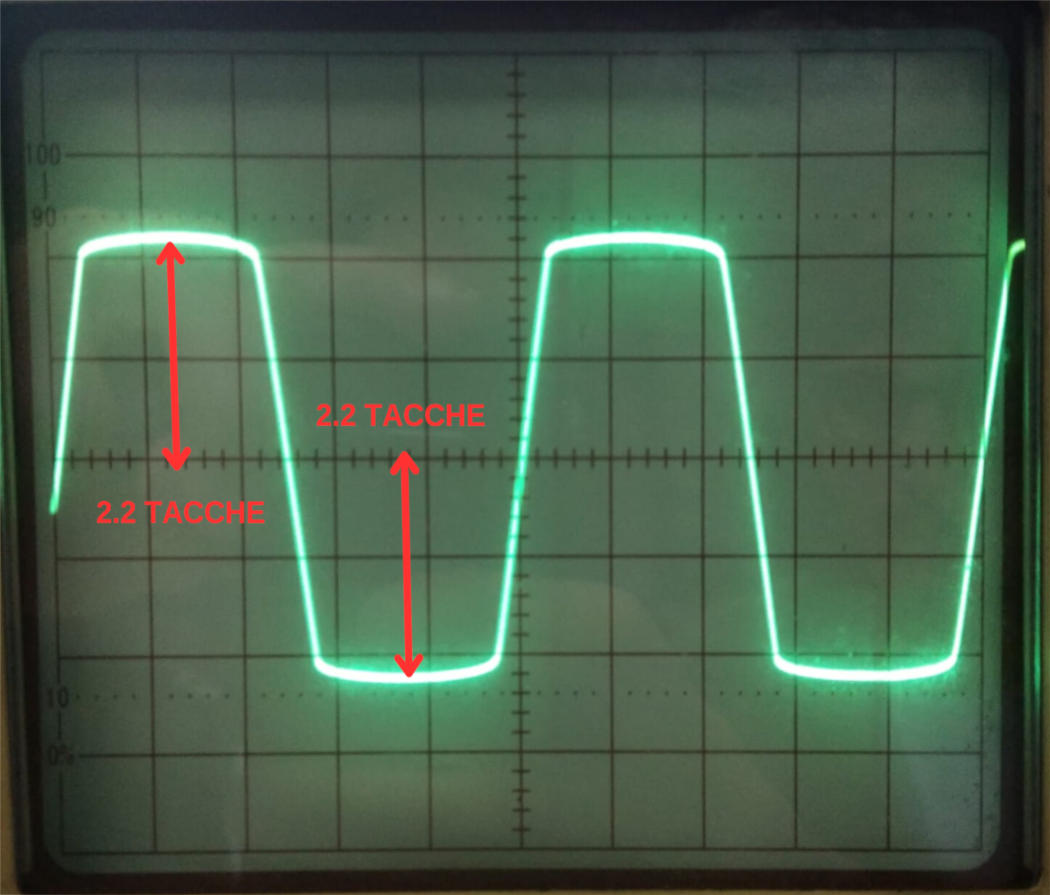
\includegraphics[width=\textwidth]{../assets/Resistenze_Uguali.png}
        \caption{\emph{Onda quadra generata con resistenze uguali.}}
        \label{fig : resistenze uguali}
      \end{subfigure}
      \hfill
      \begin{subfigure}{0.3\textwidth}
        \centering
        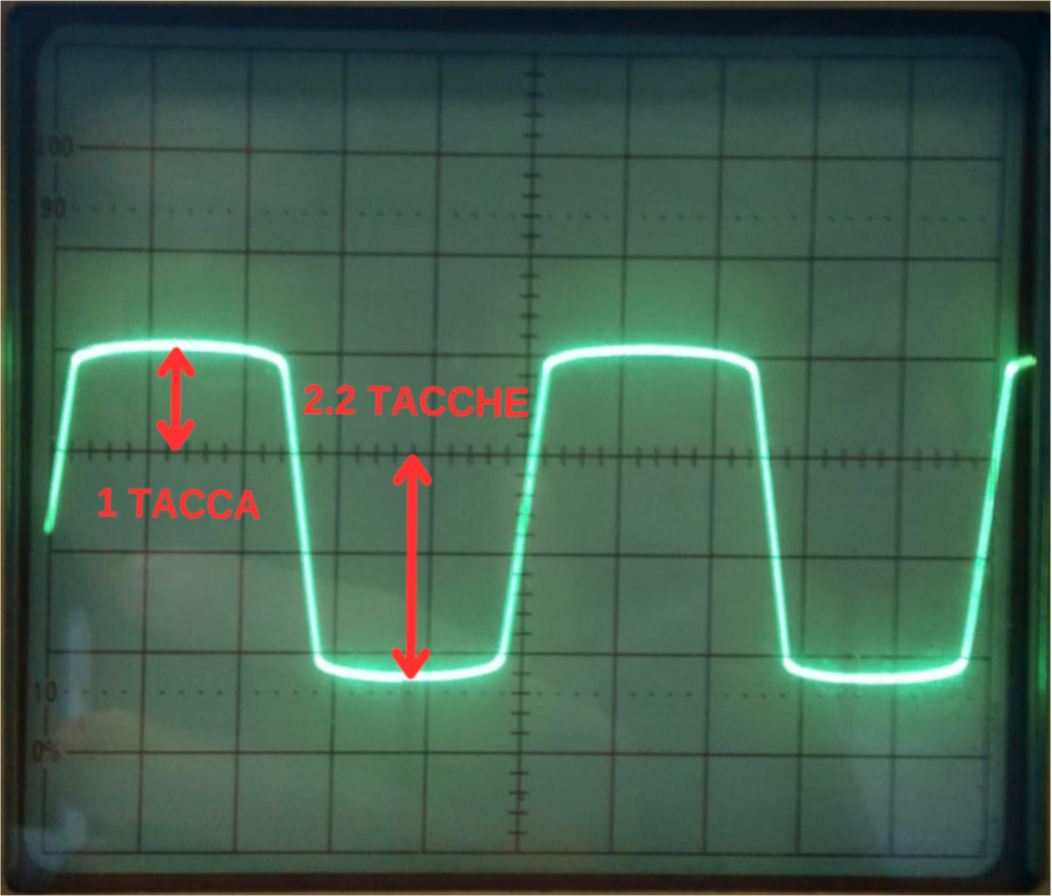
\includegraphics[width=\textwidth]{../assets/Resistenze_Diverse.png}
        \caption{\emph{Onda quadra generata variando una sola delle due resistenze.}}
        \label{fig : resistenze diverse 1}
      \end{subfigure}
      \hfill
      \begin{subfigure}{0.3\textwidth}
        \centering
        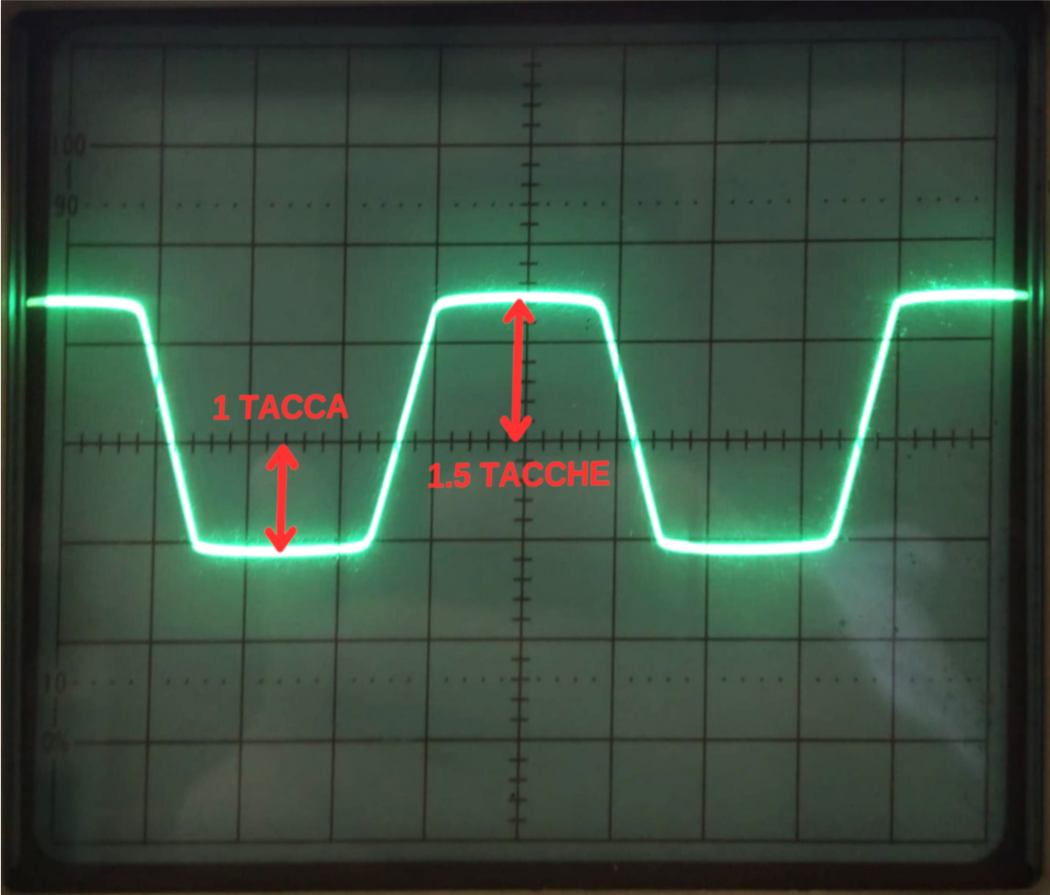
\includegraphics[width=\textwidth]{../assets/Resistenze_Diverse2.png}
        \caption{\emph{Onda quadra generata variando entrambe le resistenze.}}
        \label{fig : resistenze diverse 2}
      \end{subfigure}
      \caption{\emph{Onde quadre generate dal circuito variando i valori delle due resistenze.}}
    \label{fig : dati raccolti}
  \end{figure}

